\section{\papername}

Based on our characterization insights, we propose Splitwise, a technique to split the prompt and generation phases in the LLM inference on to separate machines.

\Cref{fig:systemdiag} shows the high-level overview of Splitwise. 
We maintain two separate pools of machines for prompt and token processing. 
A third machine pool, the mixed pool, expands and contracts as needed by the workload.
All machines are pre-loaded with the model of choice. 
When a new inference request arrives, the scheduler allocates it to a pair of machines (\ie, prompt and token).
The prompt machines are responsible for generating the first token for an input query, by processing all the input prompt tokens in the prompt phase and generating the KV-cache. 
The prompt machine also sends over the KV-cache to the token machine, which continues the token generation until the response is complete.
We use continuous batching at the token machines to maximize their utilization.
Machines in mixed pool use mixed continuous batching.

At a lower request rate, we target better latency in Splitwise, while, at a higher request rate, we target avoiding any performance or throughput reduction due to the fragmentation between prompt and token machine pools.

\begin{figure}
    \centering
    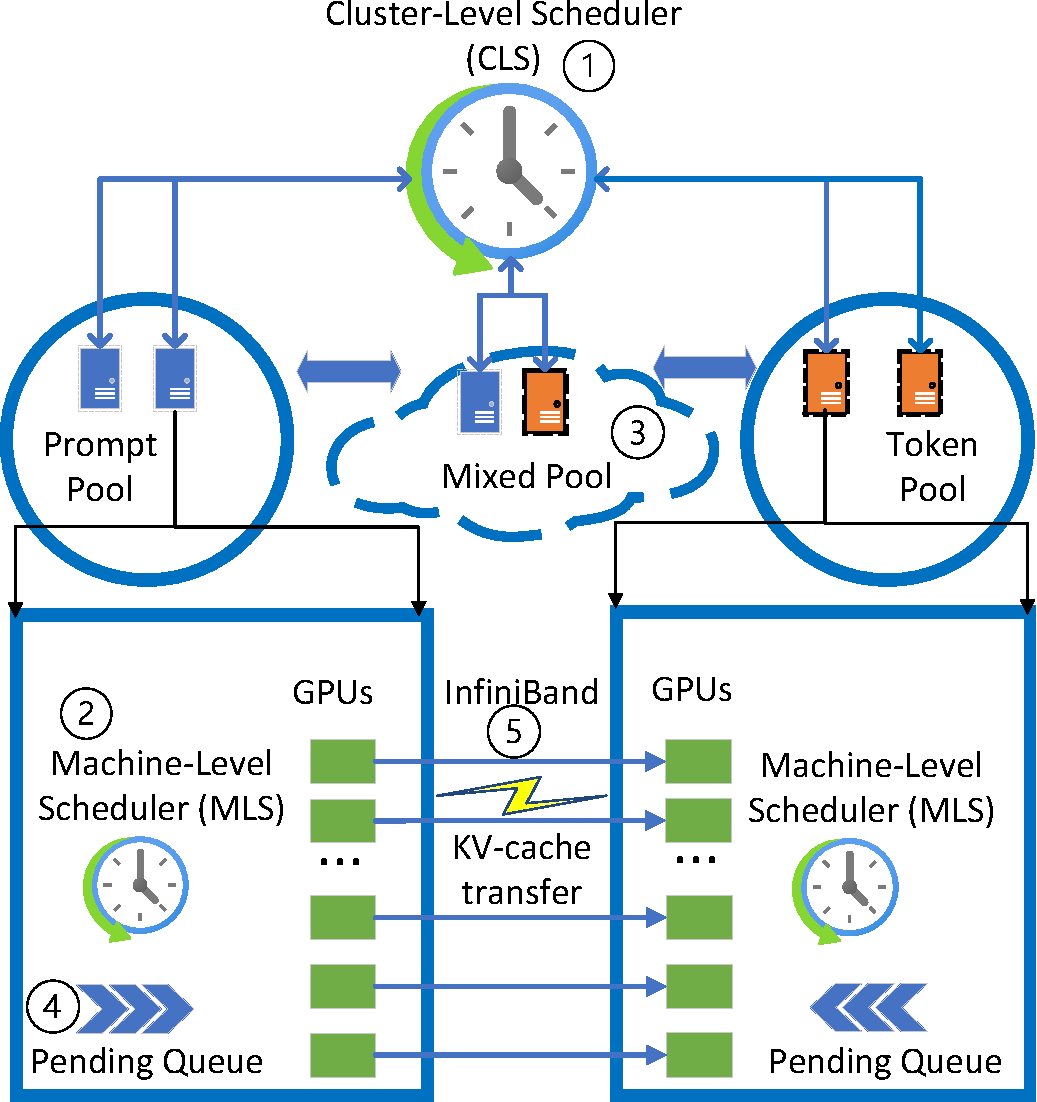
\includegraphics[width=0.8\columnwidth]{figures/design/designOverview.pdf}
    \caption{High-level system diagram of Splitwise.
    }
    \label{fig:systemdiag}
\end{figure}


Splitwise uses a hierarchical two-level scheduling as shown in \Cref{fig:systemdiag}.
The cluster-level scheduler (CLS) \circled{1} is responsible for machine pool management and for routing incoming inference requests.
The machine-level scheduler (MLS) \circled{2} maintains the pending queue and manages batching of requests at each machine.


\subsection{Cluster-level scheduling}
\label{sec:scheduler}

\myparagraph{Machine pool management}
The CLS maintains the prompt, token, and mixed machine pools \circled {3}.
Splitwise initially assigns machines to the prompt or token pool depending on the expected request load and input/output token distributions.
%\myparagraph{Mixed machine pool}
%Machines may be dynamically moved into the mixed pool to meet SLOs and avoid any performance cliffs due to fragmentation at higher loads.
Machines from the prompt or token pools may be dynamically moved into and out of the mixed pool to reduce fragmentation and meet SLOs at higher loads. 
A machine in the mixed pool retains its identity as a prompt or token machine and goes back to its original pool once there are no tasks of the opposite kind in its pending queue.
Switching pools does not incur any noticeable latency.
If the load distribution deviates considerably from initial assumptions, Splitwise employs a coarse grained \emph{re-purposing of machines} and moves machines between the prompt and token pools.
Re-purposing of machines is done infrequently, typically only if they stay in the mixed pool for a considerable amount of time.
%Re-purposing a machine could imply reloading the model (\eg, different degree of parallelism - TP or PP) which can take a significant overhead (\eg, 5 minutes).
%Therefore, this is done very infrequently if more than 10\% of the machines stay in the mixed pool for a long time threshold.
%The repurposing is performed one-by-one, and during times of lower utilization on the cluster.
%\inigo{In the rest of the paper we do not talk about the different TP/PP parallelism so moving servers between pools would be easier; we need to streamline this throughout the paper.}

\myparagraph{Request routing}
CLS uses Join the Shortest Queue (JSQ) scheduling~\cite{jsq1,jsq2} to assign a prompt and a token machine to each request.
Queue lengths are defined by the number of pending tokens.
Each machine regularly communicates to the CLS changes in its memory capacity or pending queue.
Note that this does not happen at every iteration boundary.
We simultaneously assign both the prompt and token machine when scheduling requests, since we can then overlap KV-cache transfers with prompt computation to reduce transfer overheads (\Cref{sec:designkv}).

When routing requests, if the pending queue is bigger than a certain threshold, the CLS looks for target machines in the mixed pool.
If the mixed pool is also full, it proceeds to look in the opposite pool (\ie, a token machine to run prompts and vice versa) and moves the machine into the mixed pool.
Machines in the mixed pool operate exactly as a non-Splitwise machine would, with mixed batching.
Once the queue of mixed requests is drained, the CLS transitions the machine back to its original pool.
For example, when the queue is too long, we can move a prompt machine to the mixed pool to run tokens; once the machine is done running tokens, we transition the machine back into the prompt pool.

\subsection{Machine-level scheduling}
The MLS runs on each machine and is responsible for tracking the GPU memory utilization, maintaining the pending queue \circled{4}, deciding the batch for each iteration, and reporting the relevant status to the CLS.

\myparagraph{Prompt machines}
The MLS simply uses first-come-first-serve (FCFS) to schedule prompts.
The results in \Cref{fig:char_tput_prompt} show that after 2048 prompt tokens, the throughput degrades.
For this reason, the MLS restricts the batching of multiple prompts together to 2048 tokens in total.
This is a configurable value, and can change for a different model or hardware.

\myparagraph{Token machines}
The MLS uses FCFS to schedule tokens and batches as much as possible.
\Cref{fig:char_tput_token} shows that the token generation throughput keeps scaling up with the batch size until the machine runs out of memory.
For this reason, the MLS tracks the memory and starts queueing tokens once the machine is close to running out of memory.

\myparagraph{Mixed machines}
To meet the TTFT SLO, the MLS must prioritize running prompts and schedule any new prompts in the pending queue immediately.
If the machine is running token phases and has no additional capacity to run the prompt phase, the MLS will \emph{preempt} tokens.
To avoid \emph{starvation} of the token phase due to preemption, we increase the priority of the token with age and limit the number of preemptions that each request can have.

\subsection{KV-cache transfer}
\label{sec:designkv}
As discussed in \Cref{sec:background}, the KV-cache is generated during the prompt phase of the request, and it continuously grows during the token generation phase.
In Splitwise, we need to transfer the KV-cache from the prompt machine to the token machine \circled{5} (shown in \Cref{fig:systemdiag}) to complete the inference.
This transfer delay is the main overhead associated with Splitwise.
In this section, we discuss the impact of KV-cache transfer and how we optimize it.

\begin{figure}
    \centering
     \subfloat[Serialized KV-cache transfer.]{
        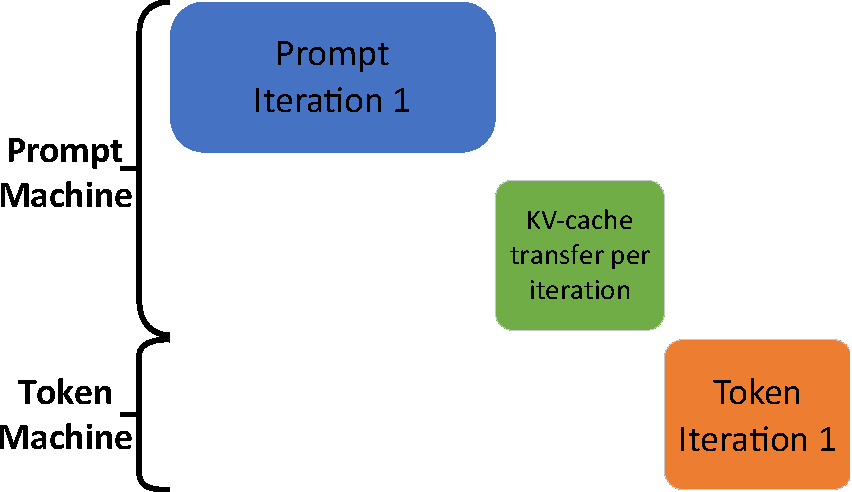
\includegraphics[width=0.46\columnwidth]{figures/design/kvcachenaive}
        \label{fig:naivekv}
    }
    \subfloat[Optimized KV-cache transfer per-layer during prompt phase.]{
        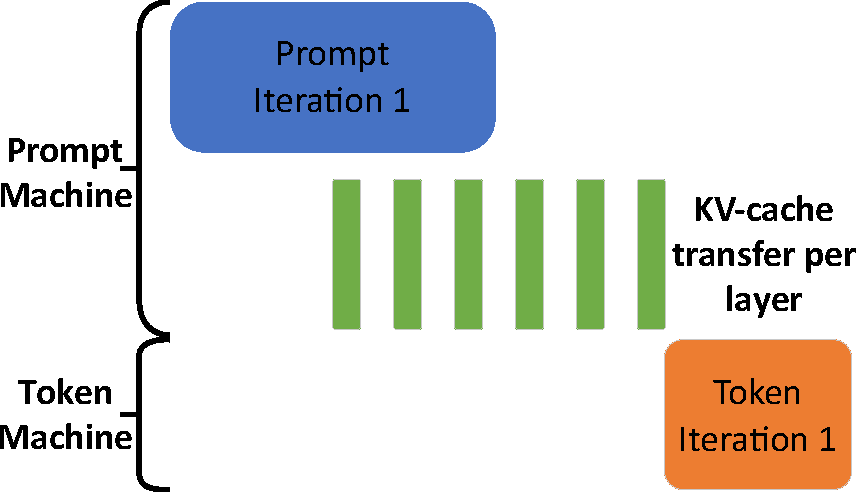
\includegraphics[width=0.46\columnwidth]{figures/design/kvcachenice}
        \label{fig:gantt_overlap}
    }
    \caption{Optimizing KV-cache transfer in Splitwise.}
    \label{fig:kvcachedesign}
\end{figure}

\Cref{fig:naivekv} shows the Gantt chart for the prompt phase, the KV-cache transfer, and the token generation phase for a single batch of requests when naively transferring the KV cache in a serialized way.
The KV-cache transfer starts only after the prompt phase has finished and the first token is generated.
Further, it needs to complete before the next output token can be generated in the token generation phase.
This directly impacts the maximum TBT and end-to-end latency of inference.

The time required for the transfer depends on the size of the KV cache (which is directly proportional to the number of prompt tokens) and on the bandwidth of the interconnect between the prompt and the token machines.
Even when using fast InfiniBand links, the \rev{transfer} overhead for large prompt sizes could become a significant fraction of the TBT.
%We discuss this further in the evaluation in \Cref{sec:expresults}.

In Splitwise, we optimize the KV-cache transfer by overlapping it with the computation in the prompt phase.
As each layer in the LLM gets calculated in the prompt machine, the KV cache corresponding to that layer is also generated.
At the end of each layer, we trigger an asynchronous transfer of the KV-cache for that layer while the prompt computation continues to the next layer.
\Cref{fig:gantt_overlap} shows this asynchronous transfer which reduces the \rev{transfer} overheads.
Layer-wise transfer also \rev{enables} other optimizations, such as earlier start of the token phase in the token machines, as well as earlier release of KV-cache memory on the prompt machines.

\rev{
Layer-wise KV-cache transfer happens in parallel with the prompt computation for the next layer.
This requires fine-grained synchronization per layer for correctness. 
Thus, it is possible to incur performance interference and increase the TTFT, especially for smaller prompts.
However, for small prompts the total KV-cache size is small and does not need the layer-wise transfer to hide the latency.
Since the number of tokens in a batch is already known at the start of computation, Splitwise picks the best technique for KV-cache transfer.
It uses serialized KV-cache transfer for smaller prompts and layer-wise transfer and for larger prompts.
We show that the overall transfer and interference overheads are relatively small in~\Cref{sec:expresults}.
}

%\inigo{Aashaka has optimizations for the layer-wise transfer which do not need require switching for short prompts.}


\begin{table*}[]
\centering
\footnotesize
\begin{tabular}{@{}cccccccc@{}}
\toprule
                      &\multicolumn{3}{c}{\textbf{Prompt Machine}} & \multicolumn{3}{c}{\textbf{Token Machine}}  &\textbf{Prompt-Token}\\
                      & \textbf{Type}   &\textbf{Cost}  &\textbf{Power}     & \textbf{Type}   &\textbf{Cost}  &\textbf{Power} &\textbf{Interconnect Bandwidth} \\\midrule                  
\textbf{Splitwise-AA}         &DGX-A100     & 1$\times$     & 1$\times$ &DGX-A100     & 1$\times$     & 1$\times$     & 1$\times$                \\
\textbf{Splitwise-HH}          &DGX-H100     & 2.35$\times$     & 1.75$\times$ &DGX-H100     & 2.5$\times$     & 1.75$\times$  & 2$\times$    \\
\textbf{Splitwise-HHcap}       &DGX-H100     & 2.35$\times$     & 1.75$\times$ &DGX-H100     & 2.5$\times$     & 1.23$\times$  & 2$\times$   \\
\textbf{Splitwise-HA}      &DGX-H100     & 2.35$\times$     & 1.75$\times$ &DGX-A100     & 1$\times$     & 1$\times$  & 1$\times$   \\
\bottomrule
\end{tabular}
\caption{Evaluated Splitwise designs all normalized to DGX-A100}
\label{tab:systems_evaluated}
\end{table*}



\subsection{Provisioning with Splitwise}
\label{sec:provision}
We leverage Splitwise to optimize LLM inference cluster deployments for power, cost, and throughput.
%It decides the type of machines and how many to provision in a cluster.

\myparagraph{Type of machines}
We propose four main variants of Splitwise-based systems:
\emph{Splitwise-AA},
\emph{Splitwise-HH},
\emph{Splitwise-HA},
and \emph{Splitwise-HHcap}.
The nomenclature is simply drawn from the first letter representing the Prompt machine type, and the second letter representing the Token machine type.
``A'' represents a DGX-A100 machine, ``H'' represents a DGX-H100 machine,
and ``Hcap'' represents a power-capped DGX-H100 machine.
\Cref{tab:systems_evaluated} shows a summary of the cost, power, and hardware in each of our evaluated systems.

Splitwise-AA uses DGX-A100 for both prompt and token pools, while Splitwise-HH uses DGX-H100 for both.
These two variants represent the commonly available setups in providers where machines are homogeneous and interchangeable.

Splitwise-HA uses DGX-H100 for the prompt pool and DGX-A100 for the token pool.
We choose this configuration based on \Cref{tab:a100h100results}, and the Insight \rom{7} (\ie, A100s can be more cost- and power-efficient for the token phase).

Splitwise-HHcap uses DGX-H100 machines for both prompt and token pools.
However, we power cap the token machines down to 70\% of their rated power, with each GPU capped by 50\% of the power.
We propose this design based on \Cref{fig:char_powercap} and Insight \rom{7} (\ie, the prompts phase is impacted by power caps while token has no performance impact with 50\% lower power cap per GPU).

\myparagraph{Number of machines}
The LLM inference cluster deployment must be sized with the appropriate number of prompt and token machines.
Our methodology involves searching the design space using our event-driven cluster simulator, which is described in detail in \Cref{sec:method}.
We need to provide as input:
(1) the target cluster design (\eg, Splitwise-HA or Splitwise-HHcap),
(2) an LLM-specific performance model that can estimate the TTFT and TBT at various input, output, and batch sizes,
(3) a short trace derived from the target prompt and token size distributions for the service (\eg, \Cref{fig:prompt_token_sizes}), 
(4) the SLOs (\eg, \Cref{tab:eval-slo}),
(5) the constraints (\eg, throughput),
and (6) the optimization goal (\eg, minimize cost).
Using this information, our provisioning framework searches the space for the desired optimal point.
For example, searching with a throughput constraint and a cost minimization goal gives us iso-throughput cost-optimized clusters across different designs. 

\begin{figure}
    \centering
    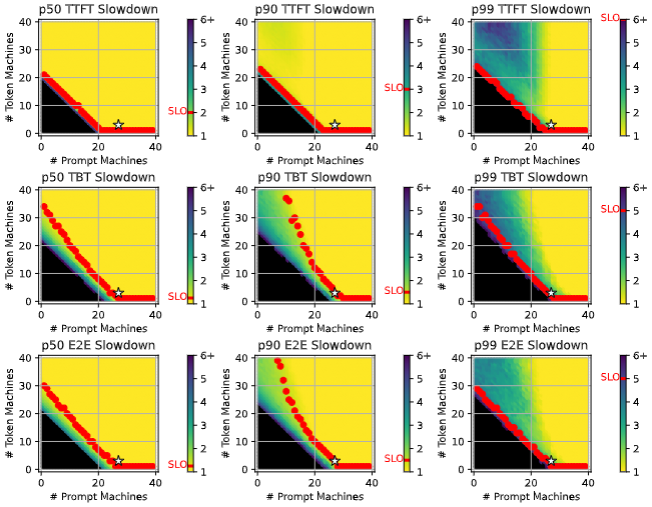
\includegraphics[width=1.0\columnwidth]{figures/design/sweep}
    \caption{Design space for provisioning a Splitwise-HH cluster.
    Cluster configurations targets a peak throughput of 70 RPS.
    The cost-optimal Splitwise-HH configuration is marked with $\star$ (27 prompt and 3 token machines).
    }
    \label{fig:provisioning}
\end{figure}


\myparagraph{Search space}
\Cref{fig:provisioning} shows an example of the two-dimensional search space for the number of prompt and token machines under Splitwise-HH for the coding workload (using a 2-minute trace).
The simulator outputs the various percentiles for TTFT, TBT, and E2E latencies.
Then, we select the clusters that meet the SLOs for each of these metrics and optimize our target function.
For example, \Cref{fig:provisioning} shows a $\star$ for the setup with 27 prompt and 3 token machines with the lowest cost that achieves 70 RPS.
We call this setup \emph{iso-throughput cost-optimized}.

\myparagraph{Optimization}
We can use three optimization goals:
\emph{throughput}, \emph{cost}, and \emph{power}.
Throughput optimization is important for both, the cloud service provider (CSP) and the user.
Cost optimization has different importance levels to the CSP and the user.
For the CSP, a higher cost for the same throughput might be acceptable if there are gains in power and space requirements for the cluster.
However, for the end-user, a higher cost at the same throughput is generally unacceptable.
Finally, power optimization is attractive for a CSP, since it enables more GPUs to be deployed in the same datacenter~\cite{patel2023polca,patel2024llmpower}, but it may not be as important to the user.
We only consider the provisioned power, and not the dynamic power utilization, in our study.

\rev{
\subsection{Practical Considerations}
\label{sec:splitwise_considerations}

\myparagraph{Accuracy impact}
Splitwise does not impact accuracy since it uses lossless KV-cache transfer and does not add any randomization.
It executes inference with the same parameters and state as on a single machine.

\myparagraph{Scalability}
Since LLM requests are much longer than typical ML requests~\cite{gujarati2020_Serving,gupta2020deeprecsys}, they incur lower scheduling overhead for similar cluster sizes. 
However, the CLS may become a scalability bottleneck for large clusters.
Insights from prior work on partitioned or replicated scheduling could help improve scalability~\cite{ousterhout2013_Sparrow,boutin2014apollo, schwarzkopf2013omega} and are orthogonal to Splitwise.

\myparagraph{Reliability and fault tolerance}
If the prompt or the token machine fail, Splitwise simply restarts requests from scratch, similar to today’s LLM serving systems~\cite{vllm,huggingface_tgi}.
Alternatively, Splitwise could checkpoint the KV-cache generated after prompt computation into an in-memory database.
To recover, Splitwise can use this cache to skip prompt recomputation, and start right away with the token phase.
The KV-cache could also be checkpointed periodically during the token phase.
Designing safe and efficient failure recovery is out of scope for our paper.
}
